\documentclass[t,xcolor={svgnames}]{beamer}
%\mode<presentation>

\setbeamertemplate{itemize items}[circle]
\setbeamertemplate{headline}{% 
  \hfill% 
  \usebeamercolor[fg]{page number in head/foot}% 
  \usebeamerfont{page number in head/foot}% 
  \insertpagenumber% 
  \kern1em\vskip-1em% 
}
\usepackage{pgfpages}
%\setbeameroption{show notes}
%\setbeameroption{show notes on second screen=right}
\usepackage{apalike}
\usepackage{graphicx} % Required for including images
\graphicspath{{figures/}} % Location of the graphics files
\usepackage{booktabs} % Top and bottom rules for table
\usepackage[font=small,labelfont=bf]{caption} % Required for specifying captions to tables and figures
\usepackage{wrapfig} % Allows wrapping text around tables and figures
\usepackage{lipsum,adjustbox}
\usepackage[absolute,overlay]{textpos}
\usepackage{url}
\usepackage{lmodern}
\usepackage{amsmath}
\usepackage{amsfonts}
\usepackage{color}
\usepackage{array}
\usepackage{multirow}
\usepackage{multicol}
\usepackage{tikz}
\usepackage{tikz-dependency}
\usetikzlibrary{arrows.meta,graphs,graphs.standard,graphdrawing,quotes,shapes}
\usegdlibrary{layered,trees}
\tikzset{
  invisible/.style={opacity=0},
  visible on/.style={alt={#1{}{invisible}}},
  alt/.code args={<#1>#2#3}{%
    \alt<#1>{\pgfkeysalso{#2}}{\pgfkeysalso{#3}} % \pgfkeysalso doesn't change the path
  },
}
\captionsetup{labelformat=empty}
\newcommand{\parser}[1]{TUPA\textsubscript{#1}}

\makeatletter
\pgfdeclareshape{vector}{
	  \inheritsavedanchors[from={rectangle}]
	  \inheritbackgroundpath[from={rectangle}]
	  \inheritanchorborder[from={rectangle}]
	  \foreach \x in {center,north east,north west,north,south,south east,south west,east,west}{
	    \inheritanchor[from={rectangle}]{\x}
	  }

    \backgroundpath{
      \pgftransformshift{\pgfpoint{-16pt}{-4pt}}
		  \draw[rounded corners=2pt] (0,0) rectangle (32pt,8pt);
    }

    \beforebackgroundpath{
      \draw[step=8pt,help lines,-] (8pt,.1pt) grid (24pt,7.9pt);
    }
}
\makeatother

\AtBeginSection[]{
  \begin{frame}
  \vfill
  \centering
  \begin{beamercolorbox}[sep=8pt,center,shadow=true,rounded=true]{title}
    \usebeamerfont{title}\insertsectionhead\par%
  \end{beamercolorbox}
  \vfill
  \end{frame}
}


\begin{document}


\title{Multitask Parsing \\ Across Semantic Representations}
\author{\textbf{Daniel Hershcovich}, Omri Abend and Ari Rappoport}
\date{June 14, 2018}

\begin{frame}
\titlepage
\end{frame}


%----------------------------------------------------------------------------------------

\begin{frame}
\frametitle{Semantic Graph Parsing}
Semantic representations:
graph structure for predicates, arguments, their attributes and relations.

Abstract away from syntactic detail that does not affect meaning.

\begin{center}
  \begin{tikzpicture}[level distance=14mm, sibling distance=15mm, ->]
  \tikzstyle{word} = [font=\rmfamily,color=black]
    \node (ROOT) [fill=blue, circle] {}
      child {node (You) [word] {You} edge from parent}
      child {node [word] {want} edge from parent}
      child {node (totakealongbath) [fill=blue, circle] {}
      {
        child {node [word] {to} edge from parent}
        child {node (takeabath) [fill=blue, circle] {}
        {
          child {node [word] {take} edge from parent}
          child {node [word] {a} edge from parent}
          child {node [word] (long) {long} edge from parent[draw=none]}
          child {node [word] {bath} edge from parent}
        } edge from parent}
      } edge from parent}
      ;
    \draw[bend left,dashed,->] (totakealongbath) to (You);
    \draw[bend left,->] (totakealongbath) to (long);
  \end{tikzpicture}
\end{center}

Semantic parsing is important for natural language understanding.
Representation schemes vary.
Data is mostly \textbf{small}, \textbf{in-domain}, and in \textbf{English}.
\end{frame}

\begin{frame}
\frametitle{Universal Conceptual Cognitive Annotation (UCCA)}
Cross-linguistically applicable \cite{abend2013universal}.
Stable in translation \cite{sulem2015conceptual}.

\vfill
English\\
\vspace{-1cm}
\begin{adjustbox}{center}
  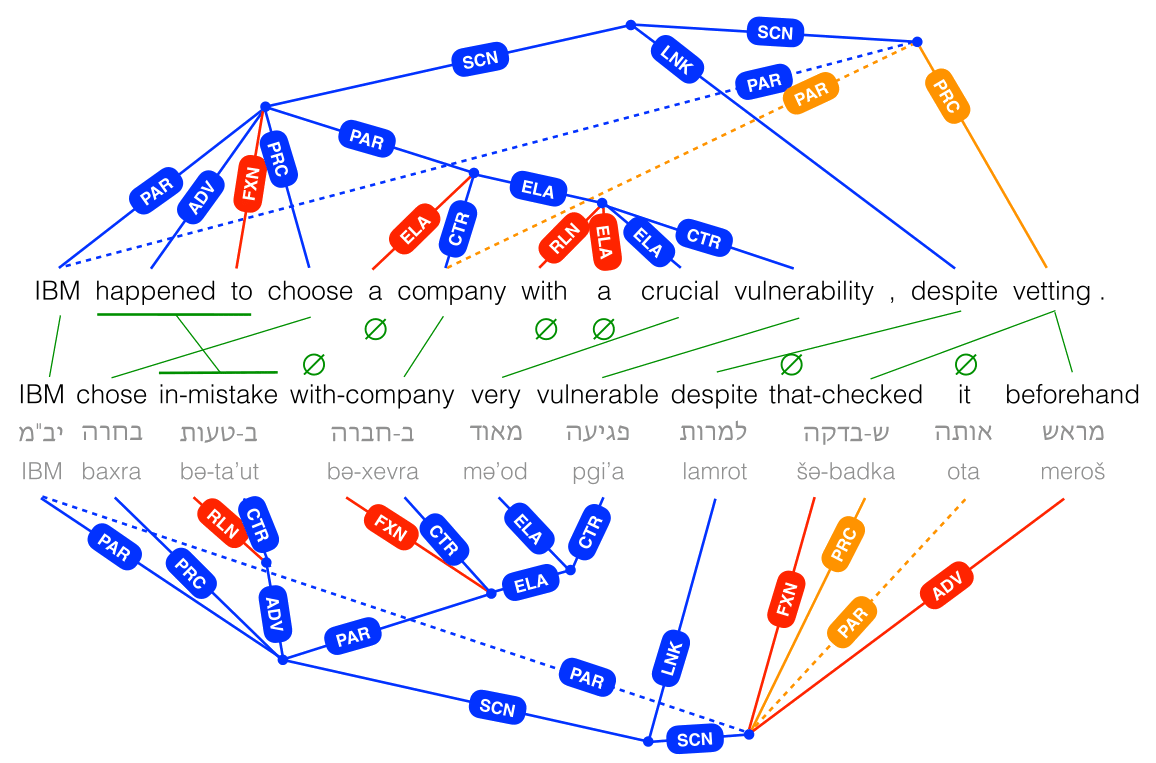
\includegraphics[width=\textwidth,height=\textheight,keepaspectratio]{crosslinguistic.png}
\end{adjustbox}
\\
\vspace{-1cm}
Hebrew
\end{frame}

\begin{frame}
\frametitle{Transition-Based Parsing}
Parse text $w_1 \ldots w_n$ to graph $G$ incrementally by applying transitions to the parser state:
stack, buffer and constructed graph.

\vfill
Initial state:
\begin{tikzpicture}[every node/.append style={font=\rmfamily}, circle]
	\draw[xstep=1cm,ystep=5mm,color=gray] (-0.01,0) grid (1,.5);
	\node[anchor=west,style={font=\sffamily}] at (-0.1,1.00)     {stack};
	\node[fill=black] at (0.5,0.25) {};
	\draw[xstep=1cm,ystep=5mm,color=gray] (3,0) grid (10,.5);
	\node[anchor=west,style={font=\sffamily}] at (8.9,1.00) {buffer};
	\node[anchor=west] at (3,0.25) {\small You};
	\node[anchor=west] at (4,0.25) {\small want};
	\node[anchor=west] at (5,0.25) {\small to};
	\node[anchor=west] at (6,0.25) {\small take};
	\node[anchor=west] at (7,0.25) {\small a};
	\node[anchor=west] at (8,0.25) {\small long};
	\node[anchor=west] at (9,0.25) {\small bath};
\end{tikzpicture}

\vfill
\parser{} transitions:

\{\textsc{Shift, Reduce, Node$_X$, Left-Edge$_X$, Right-Edge$_X$,}\\
\hspace{5mm}\textsc{Left-Remote$_X$, Right-Remote$_X$, Swap, Finish}\}

\vfill
Support {\color{blue}non-terminal nodes}, {\color{orange}reentrancy} and {\color{red}discontinuity}.
\end{frame}

\begin{frame}
\frametitle{\parser{} Model}
Learns to greedily predict transition based on current state.

BiLSTM + MLP classifier \cite{kiperwasser2016simple}.

\vfill

Features:
words, POS, syntactic dependencies, existing edge labels \\
from the stack and buffer + parents, children, grandchildren;
ordinal features (height, number of parents and children)

\vspace{5mm}
\begin{tikzpicture}
	\draw[xstep=1cm,ystep=5mm,color=gray] (-0.01,0) grid (4,.5);
	\draw[xstep=1cm,ystep=5mm,color=gray] (5,0) grid (10,.5);
	\node[anchor=west] at (-0.1,1.00) {stack};
	\node[anchor=west] at (8.9,1.00) {buffer};
	\foreach \i in {0.5,8.5,9.5} {
		\node[fill=gray, circle] at (\i,0.25) {};
	}
	\foreach \i in {1.5,2.5,3.5,5.5,6.5,7.5} {
		\node[fill=black, circle] at (\i,0.25) {};
	}
\end{tikzpicture}
\end{frame}

\begin{frame}
\centering

\onslide<2>{
\fbox{
\begin{minipage}{.5\textwidth}
\begin{tikzpicture}[every node/.append style={font=\rmfamily}]
	\node[anchor=west,style={font=\sffamily}] at (-1.2,0.25){stack};
	\draw[xstep=1cm,ystep=5mm,color=gray] (-0.01,0) grid (4,.5);
	\node[fill=black, circle] at (0.5,0.25) {};
	\node[fill=blue, circle] at (2.5,0.25) {};
	\node[anchor=west] at (1,0.25) {\small You};
	\node[anchor=west] at (3,0.25) {\small take};
\end{tikzpicture}

\vspace{1cm}
\begin{tikzpicture}[every node/.append style={font=\rmfamily}]
	\node[anchor=west,style={font=\sffamily}] at (3.8,0.25){buffer};
	\draw[xstep=1cm,ystep=5mm,color=gray] (5,0) grid (9,.5);
	\node[fill=red, circle] at (5.5,0.25) {};
	\node[anchor=west] at (6,0.25) {\small a};
	\node[anchor=west] at (7,0.25) {\small long};
	\node[anchor=west] at (8,0.25) {\small bath};
\end{tikzpicture}
\end{minipage}
\begin{minipage}{.4\textwidth}
\scalebox{.8}{
\begin{tikzpicture}[level distance=1cm, sibling distance=1cm, ->,
    every node/.append style={font=\rmfamily}]
    \node[anchor=west,style={font=\sffamily}] at (5,0) {graph};
    \draw[color=gray] (1.2,.3) rectangle (4.9,-3.2);
    \node(ROOT)[fill=black, circle, visible on=<2->] at (3,0) {}
      child {node (You) {You} edge from parent node [left] {\scriptsize $A$}}
      child {node {want} edge from parent node [left] {\scriptsize $P$}}
      child {node (totakealongbath) [fill=blue, circle] {}
      {
        child {node {to} edge from parent node [left] {\scriptsize $F$}}
        child {node (takeabath) [fill=red, circle] {}
        {
          child {node {take} edge from parent node [right] {\scriptsize $C$}}
          child [opacity=0] {node {a} edge from parent node [right] {\scriptsize $F$}}
          child [opacity=0] {node (long) {long} edge from parent [draw=none]}
          child [opacity=0] {node {bath} edge from parent node [right] {\scriptsize $C$}}
        } edge from parent [draw=none]}
      } edge from parent [draw=none]}
      ;
\end{tikzpicture}
}
\end{minipage}
}
}

\scalebox{.7}{
\begin{tikzpicture}[->]
	\tiny
	\tikzstyle{main}=[circle, minimum size=7mm, draw=black!80, node distance=12mm]
	\foreach \i/\word in {1/{You},3/{want},5/{to},7/{take},9/{a},11/{long},13/{bath}} {
	    \node (x\i) at (\i,-1.3) {\Large\textrm\word};
	    \node[main, fill=white!100] (h\i) at (\i,0) {LSTM};
        \path (x\i) edge (h\i);
	    \node[main, fill=white!100] (i\i) at (\i.5,.8) {LSTM};
        \path (x\i) edge [bend right] (i\i);
	    \node[main, fill=white!100] (l\i) at (\i.5,2.3) {LSTM};
        \path (h\i) edge [bend left] (l\i);
        \path (i\i) edge (l\i);
	    \node[main, fill=white!100] (k\i) at (\i,3.1) {LSTM};
        \path (i\i) edge [bend left] (k\i);
        \path (h\i) edge [bend left] (k\i);
	}
	\foreach \current/\next in {1/3,3/5,5/7,7/9,9/11,11/13} {
        \path (h\current) edge (h\next);
        \path (i\next) edge (i\current);
        \path (l\current) edge (l\next);
        \path (k\next) edge (k\current);
	}
    \onslide<2>\node[main, fill=white!100] (mlp) at (7,4.6) {MLP};
	\onslide<2>\foreach \i in {5,7,9} {
        \path (l\i) edge (mlp);
        \path (k\i) edge (mlp);
    }
    \coordinate (state) at (10.5,6.5);
    \onslide<2>\path (state) edge [bend left] (mlp);
    \onslide<2>\node (transition) at (7,5.8) {\large\textsc{Node}$_C$};
    \onslide<2>\path (mlp) edge (transition);
\end{tikzpicture}
}
\end{frame}

\begin{frame}
\frametitle{Multitask Parsing}
We consider four schemes \cite{abend2013universal,banarescu2013abstract,oepen2016towards,nivre2016universal}:

	{
	\hfill
	  \color{Indigo}
	    \scalebox{.6}{
	    \begin{tikzpicture}[level distance=15mm, -{Latex[length=2mm]},
	        every node/.append style={font=\bf\ttfamily},
	        every circle node/.append style={fill=Indigo},
	      level 1/.style={sibling distance=29mm},
	      level 2/.style={sibling distance=18mm}]
	      \tikzstyle{word} = [font=\rmfamily,color=black]
	      \node[font=\bf\sffamily\Large] at (-4,0) {UCCA:};
      \node (ROOT) [circle] {}
        child {node (After) [word] {After} edge from parent node[above] {L}}
        child {node (graduation) [circle] {}
        {
          child {node [word] {graduation} edge from parent node[left] {P}}
        } edge from parent node[right] {H} }
        child {node [word] {,} edge from parent node[below] {U}}
        child {node (moved) [circle] {}
        {
          child {node (John) [word] {John} edge from parent node[left] {A}}
          child {node [word] {moved} edge from parent node[left] {P}}
          child {node [circle] {}
          {
            child {node [word] {to} edge from parent node[left] {R}}
            child {node [word] {Paris} edge from parent node[right] {C}}
          } edge from parent node[above] {A} }
        } edge from parent node[above] {H} }
        ;
      \draw[dashed,-{Latex[length=5mm]}] (graduation) to node [above] {A} (John);
	    \end{tikzpicture}
	    }
	}
	
	\vspace{-14mm}
	\hspace{-9mm}
	\scalebox{.9}{
	  \begin{tikzpicture}[-{Latex[length=2mm]}, color=DarkGreen, level distance=16mm,
	      every node/.append style={sloped,anchor=south,auto=false,font=\scriptsize\bf\ttfamily},
	      level 1/.style={sibling distance=24mm}]
	    \node[font=\bf\sffamily\small] at (-2.6,0) {AMR:};
    \node (ROOT) [ellipse] {move-01}
      child {node [ellipse] {after}
      {
            child {node (graduation) [ellipse] {graduate-01} edge from parent node {op1} }
      } edge from parent node {time} }
      child {node (John) [ellipse] {person}
      {
        child {node [ellipse] {name}
        {
            child {node [ellipse] {"John"} edge from parent node {op1} }
        } edge from parent node {name} }
      } edge from parent node {ARG0} }
      child {node [ellipse] {city}
      {
        child {node [ellipse] {name}
        {
            child {node [ellipse] {"Paris"} edge from parent node {op1} }
        } edge from parent node {name} }
      } edge from parent node {ARG2} }
      ;
      \draw (graduation) to node {ARG0} (John);
	  \end{tikzpicture}
	  }
	\vspace{-24mm}
	
	\begin{center}
	\hspace{2cm}{\color{NavyBlue}\bf\sffamily\scriptsize UD:}
	\end{center}
	
	\vspace{-9mm}
	
	\begin{flushright}
	\begin{minipage}{.5\textwidth}
	    \rmfamily
	    \scalebox{.7}{
	    \begin{dependency}[edge style={-{Latex[length=2mm]}, color=NavyBlue},
	        text only label, label style={above, color=NavyBlue, font=\bf\ttfamily}, font=\small]
	    \begin{deptext}[column sep=.8em,ampersand replacement=\^]
    After \^ graduation \^ , \^ John \^ moved \^ to \^ Paris \\
    \end{deptext}
        \depedge[edge unit distance=1em]{2}{1}{case}
        \depedge[edge unit distance=1em]{4}{3}{punct}
        \depedge[edge unit distance=1em, edge start x offset=-4mm]{5}{4}{nsubj}
        \depedge[edge unit distance=1em, edge end x offset=-3mm]{2}{5}{obl}
        \depedge[edge unit distance=1em]{7}{6}{case}
        \deproot[edge unit distance=1em]{5}{root}
        \depedge[edge unit distance=1.5em, edge start x offset=1mm]{5}{7}{obl}
    \end{dependency}
	}
	\end{minipage}
	
	\begin{minipage}{.06\textwidth}
	{\color{DarkRed}\bf\sffamily\scriptsize SDP:}
	\end{minipage}
	\begin{minipage}{.5\textwidth}
	    \rmfamily
	    \scalebox{.7}{
	    \begin{dependency}[edge style={-{Latex[length=2mm]}, color=DarkRed},
	        text only label, label style={above, color=DarkRed, font=\bf\ttfamily}, font=\small]
	    \begin{deptext}[column sep=.8em,ampersand replacement=\^]
    After \^ graduation \^ , \^ John \^ moved \^ to \^ Paris \\
    \end{deptext}
        \depedge[edge unit distance=1em]{1}{2}{ARG2}
        \depedge[edge unit distance=1em, edge start x offset=-4mm]{5}{4}{ARG1}
        \depedge[edge unit distance=1em, edge end x offset=-3mm]{1}{5}{ARG1}
        \deproot[edge unit distance=1.25em]{5}{top}
        \depedge[edge unit distance=2em, edge start x offset=1mm, edge end x offset=3mm]{5}{7}{ARG2}
        \depedge[edge unit distance=1em, edge end x offset=5mm]{6}{5}{ARG1}
        \depedge[edge unit distance=1em]{6}{7}{ARG2}
    \end{dependency}
	}
	\end{minipage}
	\end{flushright}
	
\end{frame}


\begin{frame}
\frametitle{Experimental Setup}
\begin{itemize}
 \item UCCA Wikipedia corpus ($\stackrel{\text{train}}{4268}+\stackrel{\text{dev}}{454}+\stackrel{\text{test}}{503}$ sentences).
 \item Out-of-domain: English part of English-French parallel corpus,
 	\textit{Twenty Thousand Leagues Under the Sea} (506 sentences).
\end{itemize}

\vfill
\begin{center}
  \begin{minipage}{.3\textwidth}
\includegraphics[width=\textwidth]{wikipedia.png}\end{minipage}
  \begin{minipage}{.3\textwidth}
\includegraphics[width=\textwidth]{squid.jpg}\end{minipage}
\end{center}
\end{frame}

\begin{frame}
\frametitle{Data}
\centering
\begin{tabular}{l|ccc|c}
	& \multicolumn{3}{c|}{Wiki} & 20K \\
	& \small Train & \small Dev & \small Test & Leagues \\
	\hline
	\# passages & 300 & 34 & 33 & 154 \\
	\# sentences & 4268 & 454 & 503 & 506 \\
	\hline
	\# nodes & 298,993 & 33,704 & 35,718 & 29,315 \\
	\% terminal & 42.96 & 43.54 & 42.87 & 42.09 \\
	\% non-term. & 58.33 & 57.60 & 58.35 & 60.01 \\
	\% \textbf{discont.} & \textbf{0.54} & \textbf{0.53} & \textbf{0.44} & \textbf{0.81} \\
	\% \textbf{reentrant} & \textbf{2.38} & \textbf{1.88} & \textbf{2.15} & \textbf{2.03} \\
	\hline
	\# edges & 287,914 & 32,460 & 34,336 & 27,749 \\
	\% primary & 98.25 & 98.75 & 98.74 & 97.73 \\
	\% remote & 1.75 & 1.25 & 1.26 & 2.27 \\
	\hline
	\multicolumn{3}{l}{\footnotesize Average per non-terminal node} \\
	\# children & 1.67 & 1.68 & 1.66 & 1.61 
\end{tabular}
\captionof{table}{Corpus statistics.}
\end{frame}

\begin{frame}
\frametitle{Evaluation}
Comparing graphs over the same sequence of tokens,
\begin{itemize}
\item Match edges by their terminal yield and label.
\item Calculate \textbf{labeled precision, recall and F1} scores.
\item Separate primary and remote edges.
\end{itemize}
\vfill
\begin{adjustbox}{frame,scale=.75,center}
	\begin{tikzpicture}[level distance=15mm, sibling distance=15mm, ->,
	    every circle node/.append style={fill=black}]
	  \tikzstyle{word} = [font=\rmfamily,color=black]
	  \node at (-1,.7) {gold};
	  \node (ROOT) at (0,0) [circle] {}
	    child {node (After) [word] {After} edge from parent node[left] {$L$}}
	    child {node (graduation) [circle] {}
	    {
	      child {node [word] {graduation} edge from parent node[left] {$P$}}
	    } edge from parent node[left] {$H$} }
	    child {node [word] {,} edge from parent node[right] {$U$}}
	    child {node (moved) [circle] {}
	    {
	      child {node (Joe) [word] {Joe} edge from parent node[left] {$A$}}
	      child {node [word] {moved} edge from parent node[left] {$P$}}
	      child {node [circle] {}
	      {
	        child {node [word] {to} edge from parent node[left] {$R$}}
	        child {node [word] {Paris} edge from parent node[right] {$C$}}
	      } edge from parent node[right] {$A$} }
	    } edge from parent node[right] {$H$} }
	    ;
	  \draw[dashed,->] (graduation) to node [auto] {$A$} (Joe);
	  \node at (6,.7) {predicted};
	  \node (ROOT_) at (7,0) [circle] {}
	    child {node (After_) [word] {After} edge from parent node[left] {$L$}}
	    child {node (graduation_) [circle] {}
	    {
	      child[red] {node [word] {graduation} edge from parent node[left] {$S$}}
	    } edge from parent node[left] {$H$} }
	    child {node [word] {,} edge from parent node[right] {$U$}}
	    child {node (moved) [circle,xshift=3mm,yshift=-7mm] {}
	    {
	      child {node (Joe_) [word] {Joe} edge from parent node[left] {$A$}}
	      child {node [word] {moved} edge from parent node[left] {$P$}}
	      child[red] {node [word] {to} edge from parent node[left] {$F$}}
	      child[red] {node (Paris_) [word] {Paris} edge from parent node[right] {$A$}}
	    } edge from parent node[right] {$H$} }
	    ;
	  \draw[bend left,dashed,->] (graduation_) to node [auto] {$A$} (Joe_);
	  \draw[bend left,dashed,->,red] (graduation_) to node [auto] {$A$} (Paris_);
	\end{tikzpicture}
\end{adjustbox}
\vfill
\begin{adjustbox}{scale=.75,center}
	Primary:
	\begin{tabular}{ccc}
		\textbf{LP} & \textbf{LR} & \textbf{LF} \\ \hline
		$\frac69=67\%$ & $\frac6{10}=60\%$ & 64\%
	\end{tabular}
	\hspace{1cm}
	Remote:
	\begin{tabular}{ccc}
		\textbf{LP} & \textbf{LR} & \textbf{LF} \\ \hline
		$\frac12=50\%$ & $\frac11=100\%$ & 67\%
	\end{tabular}
\end{adjustbox}
\end{frame}

\begin{frame}
\frametitle{Results}
\parser{BiLSTM} obtains the highest F-scores in all metrics:
\begin{center}
	\begin{tabular}{l|ccc|ccc}
		& \multicolumn{3}{c|}{Primary edges} & \multicolumn{3}{c}{Remote edges} \\
		& \textbf{LP} & \textbf{LR} & \textbf{LF} & \textbf{LP} & \textbf{LR} & \textbf{LF} \\
		\hline
		\parser{Sparse}
		& 64.5 & 63.7 & 64.1 & 19.8 & 13.4 & 16 \\
		\parser{MLP}
		& 65.2 & 64.6 & 64.9 & 23.7 & 13.2 & 16.9 \\
		\parser{BiLSTM}
		& 74.4 & 72.7 & \textbf{73.5} & 47.4 & 51.6 & \textbf{49.4} \\
		\hline
		\scriptsize Bilexical DAG
		& & & \scriptsize (91) & & & \scriptsize (58.3) \\
		DAGParser
		& 61.8 & 55.8 & 58.6 & 9.5 & 0.5 & 1 \\
		TurboParser
		& 57.7 & 46 & 51.2 & 77.8 & 1.8 & 3.7 \\
		\hline
		\scriptsize Bilexical tree
		& & & \scriptsize (91) & & & \scriptsize -- \\
		MaltParser
		& 62.8 & 57.7 & 60.2 & -- & -- & -- \\
		Stack LSTM
		& 73.2 & 66.9 & 69.9 & -- & -- & -- \\
		\hline
		\scriptsize Tree
		& & & \scriptsize (100) & & & \scriptsize -- \\
		\textsc{uparse}
		& 60.9 & 61.2 & 61.1 & -- & -- & --
	\end{tabular}
	\captionof{table}{Results on the Wiki test set.}
\end{center}
\end{frame}
\note{The experiments show \parser{} outperforms a large variety of baseline parsers. \\
Remote edges are challenging -- they incorporate the REENTRANCY in the graph, and \parser{} parses them quite effectively.}

\begin{frame}
\frametitle{Results}
Comparable on out-of-domain test set:
\begin{center}
	\begin{tabular}{l|ccc|ccc}
		& \multicolumn{3}{c|}{Primary edges} & \multicolumn{3}{c}{Remote edges} \\
		& \textbf{LP} & \textbf{LR} & \textbf{LF} & \textbf{LP} & \textbf{LR} & \textbf{LF} \\
		\hline
		\parser{Sparse}
		& 59.6 & 59.9 & 59.8 & 22.2 & 7.7 & 11.5 \\
		\parser{MLP}
		& 62.3 & 62.6 & 62.5 & 20.9 & 6.3 & 9.7 \\
		\parser{BiLSTM}
		& 68.7 & 68.5 & \textbf{68.6} & 38.6 & 18.8 & \textbf{25.3} \\
		\hline
		\scriptsize Bilexical DAG
		& & & \scriptsize (91.3) & & & \scriptsize (43.4) \\
		DAGParser
		& 56.4 & 50.6 & 53.4 & -- & 0 & 0 \\
		TurboParser
		& 50.3 & 37.7 & 43.1 & 100 & 0.4 & 0.8 \\
		\hline
		\scriptsize Bilexical tree
		& & & \scriptsize (91.3) & & & \scriptsize -- \\
		MaltParser
		& 57.8 & 53 & 55.3 & -- & -- & -- \\
		Stack LSTM
		& 66.1 & 61.1 & 63.5 & -- & -- & -- \\
		\hline
		\scriptsize Tree
		& & & \scriptsize (100) & & & \scriptsize -- \\
		\textsc{uparse}
		& 52.7 & 52.8 & 52.8 & -- & -- & --
	\end{tabular}
	\captionof{table}{Results on the 20K Leagues out-of-domain set.}
\end{center}
\end{frame}
\note{We also evaluated all parsers on the out-of-domain set, to test their domain adaptation ability. The results are quite good, despite the different genre.}



\begin{frame}
\frametitle{Conclusion}
\begin{itemize}
 \item UCCA's semantic distinctions require a graph structure including {\color{blue}non-terminals}, {\color{orange}reentrancy} and {\color{red}discontinuity}.
 \item \parser{} is an accurate transition-based UCCA parser,
 	and the \textbf{first} to support UCCA and any DAG over the text tokens.
 \item Outperforms strong conversion-based baselines.
\end{itemize}

\end{frame}



\begin{frame}[allowframebreaks]
\frametitle{References}
\bibliographystyle{apalike}
\tiny\bibliography{references}
\end{frame}

\end{document}
